\documentclass{standalone}
\usepackage{tikz}
\usetikzlibrary{patterns, positioning}


\begin{document}
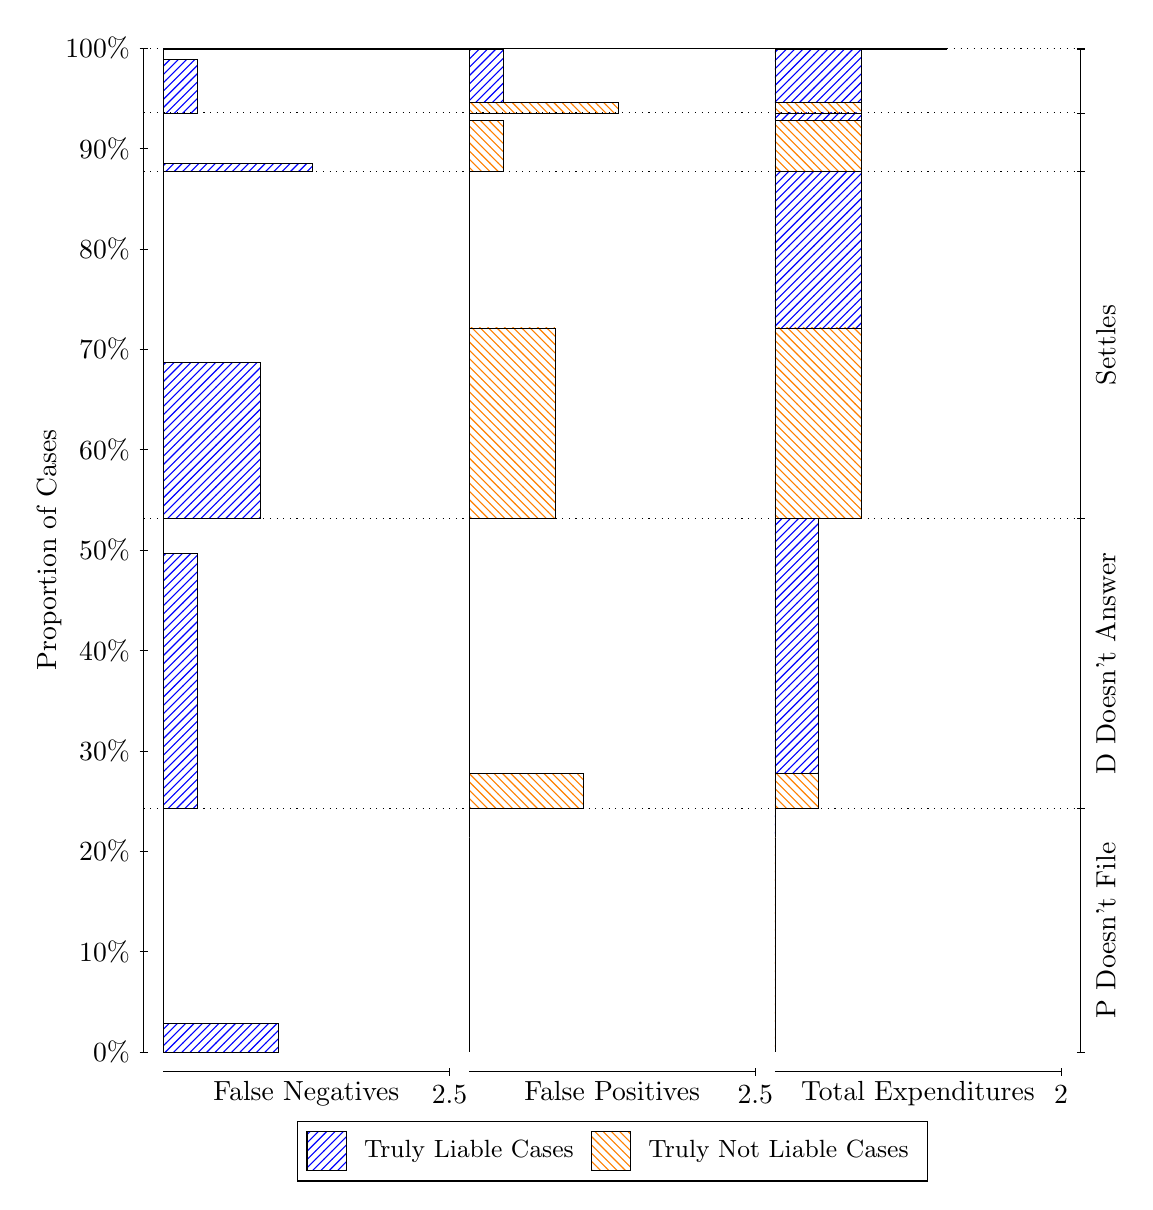
\begin{tikzpicture}
\draw[black, very thin] (1.5,1.75) -- (1.5,14.5);
\node[rotate=90, text=black, anchor=center] at (0.3, 8.125) {Proportion of Cases};
\draw[black, very thin] (1.45,1.75) -- (1.55,1.75);
\node[text=black, anchor=east] at (1.45, 1.75) {0\%};
\draw[black, very thin] (1.45,3.025) -- (1.55,3.025);
\node[text=black, anchor=east] at (1.45, 3.025) {10\%};
\draw[black, very thin] (1.45,4.3) -- (1.55,4.3);
\node[text=black, anchor=east] at (1.45, 4.3) {20\%};
\draw[black, very thin] (1.45,5.575) -- (1.55,5.575);
\node[text=black, anchor=east] at (1.45, 5.575) {30\%};
\draw[black, very thin] (1.45,6.85) -- (1.55,6.85);
\node[text=black, anchor=east] at (1.45, 6.85) {40\%};
\draw[black, very thin] (1.45,8.125) -- (1.55,8.125);
\node[text=black, anchor=east] at (1.45, 8.125) {50\%};
\draw[black, very thin] (1.45,9.4) -- (1.55,9.4);
\node[text=black, anchor=east] at (1.45, 9.4) {60\%};
\draw[black, very thin] (1.45,10.675) -- (1.55,10.675);
\node[text=black, anchor=east] at (1.45, 10.675) {70\%};
\draw[black, very thin] (1.45,11.95) -- (1.55,11.95);
\node[text=black, anchor=east] at (1.45, 11.95) {80\%};
\draw[black, very thin] (1.45,13.225) -- (1.55,13.225);
\node[text=black, anchor=east] at (1.45, 13.225) {90\%};
\draw[black, very thin] (1.45,14.5) -- (1.55,14.5);
\node[text=black, anchor=east] at (1.45, 14.5) {100\%};

\draw[black, very thin] (13.4,1.75) -- (13.4,14.5);
\draw[black, very thin] (13.35,1.75) -- (13.45,1.75);
\node[anchor=west] at (13.35, 1.75) {};
\draw[black, very thin] (13.35,4.8413) -- (13.45,4.8413);
\node[anchor=west] at (13.35, 4.8413) {};
\draw[black, very thin] (13.35,8.5229) -- (13.45,8.5229);
\node[anchor=west] at (13.35, 8.5229) {};
\draw[black, very thin] (13.35,12.931) -- (13.45,12.931);
\node[anchor=west] at (13.35, 12.931) {};
\draw[black, very thin] (13.35,13.677) -- (13.45,13.677);
\node[anchor=west] at (13.35, 13.677) {};
\draw[black, very thin] (13.35,14.489) -- (13.45,14.489);
\node[anchor=west] at (13.35, 14.489) {};
\draw[black, very thin] (13.35,14.495) -- (13.45,14.495);
\node[anchor=west] at (13.35, 14.495) {};
\draw[black, very thin] (13.35,14.5) -- (13.45,14.5);
\node[anchor=west] at (13.35, 14.5) {};

\draw[black, very thin, pattern color=blue, pattern=north east lines] (1.75,1.75) rectangle (3.2033,2.1145);
\draw[black, very thin, pattern color=orange, pattern=north west lines] (1.75,2.1145) rectangle (1.75,4.8413);
\draw[black, very thin, pattern color=blue, pattern=north east lines] (1.75,4.8413) rectangle (2.186,8.0803);
\draw[black, very thin, pattern color=orange, pattern=north west lines] (1.75,8.0803) rectangle (1.75,8.5229);
\draw[black, very thin, pattern color=blue, pattern=north east lines] (1.75,8.5229) rectangle (2.9853,10.509);
\draw[black, very thin, pattern color=orange, pattern=north west lines] (1.75,10.509) rectangle (1.75,12.931);
\draw[black, very thin, pattern color=blue, pattern=north east lines] (1.75,12.931) rectangle (3.6393,13.031);
\draw[black, very thin, pattern color=orange, pattern=north west lines] (1.75,13.031) rectangle (1.75,13.677);
\draw[black, very thin, pattern color=blue, pattern=north east lines] (1.75,13.677) rectangle (2.186,14.357);
\draw[black, very thin, pattern color=orange, pattern=north west lines] (1.75,14.357) rectangle (1.75,14.489);
\draw[black, very thin, pattern color=blue, pattern=north east lines] (1.75,14.489) rectangle (5.8193,14.491);
\draw[black, very thin, pattern color=orange, pattern=north west lines] (1.75,14.491) rectangle (1.75,14.495);
\draw[black, very thin, pattern color=orange, pattern=north west lines] (1.75,14.495) rectangle (1.75,14.497);
\draw[black, very thin, pattern color=blue, pattern=north east lines] (1.75,14.497) rectangle (1.75,14.5);
\draw[black, very thin, pattern color=orange, pattern=north west lines] (5.6333,1.75) rectangle (5.6333,4.4768);
\draw[black, very thin, pattern color=blue, pattern=north east lines] (5.6333,4.4768) rectangle (5.6333,4.8413);
\draw[black, very thin, pattern color=orange, pattern=north west lines] (5.6333,4.8413) rectangle (7.0867,5.2839);
\draw[black, very thin, pattern color=blue, pattern=north east lines] (5.6333,5.2839) rectangle (5.6333,8.5229);
\draw[black, very thin, pattern color=orange, pattern=north west lines] (5.6333,8.5229) rectangle (6.7233,10.945);
\draw[black, very thin, pattern color=blue, pattern=north east lines] (5.6333,10.945) rectangle (5.6333,12.931);
\draw[black, very thin, pattern color=orange, pattern=north west lines] (5.6333,12.931) rectangle (6.0693,13.578);
\draw[black, very thin, pattern color=blue, pattern=north east lines] (5.6333,13.578) rectangle (5.6333,13.677);
\draw[black, very thin, pattern color=orange, pattern=north west lines] (5.6333,13.677) rectangle (7.5227,13.809);
\draw[black, very thin, pattern color=blue, pattern=north east lines] (5.6333,13.809) rectangle (6.0693,14.489);
\draw[black, very thin, pattern color=orange, pattern=north west lines] (5.6333,14.489) rectangle (5.6333,14.493);
\draw[black, very thin, pattern color=blue, pattern=north east lines] (5.6333,14.493) rectangle (5.6333,14.495);
\draw[black, very thin, pattern color=orange, pattern=north west lines] (5.6333,14.495) rectangle (9.7027,14.497);
\draw[black, very thin, pattern color=blue, pattern=north east lines] (5.6333,14.497) rectangle (8.2493,14.5);
\draw[black, very thin, pattern color=orange, pattern=north west lines] (9.5167,1.75) rectangle (9.5167,4.4768);
\draw[black, very thin, pattern color=blue, pattern=north east lines] (9.5167,4.4768) rectangle (9.5167,4.8413);
\draw[black, very thin, pattern color=orange, pattern=north west lines] (9.5167,4.8413) rectangle (10.062,5.2839);
\draw[black, very thin, pattern color=blue, pattern=north east lines] (9.5167,5.2839) rectangle (10.062,8.5229);
\draw[black, very thin, pattern color=orange, pattern=north west lines] (9.5167,8.5229) rectangle (10.607,10.945);
\draw[black, very thin, pattern color=blue, pattern=north east lines] (9.5167,10.945) rectangle (10.607,12.931);
\draw[black, very thin, pattern color=orange, pattern=north west lines] (9.5167,12.931) rectangle (10.607,13.578);
\draw[black, very thin, pattern color=blue, pattern=north east lines] (9.5167,13.578) rectangle (10.607,13.677);
\draw[black, very thin, pattern color=orange, pattern=north west lines] (9.5167,13.677) rectangle (10.607,13.809);
\draw[black, very thin, pattern color=blue, pattern=north east lines] (9.5167,13.809) rectangle (10.607,14.489);
\draw[black, very thin, pattern color=orange, pattern=north west lines] (9.5167,14.489) rectangle (11.697,14.493);
\draw[black, very thin, pattern color=blue, pattern=north east lines] (9.5167,14.493) rectangle (11.697,14.495);
\draw[black, very thin, pattern color=orange, pattern=north west lines] (9.5167,14.495) rectangle (11.697,14.497);
\draw[black, very thin, pattern color=blue, pattern=north east lines] (9.5167,14.497) rectangle (11.697,14.5);
\draw[black, dotted] (1.5,4.8413) -- (13.4,4.8413);
\draw[black, dotted] (1.5,8.5229) -- (13.4,8.5229);
\draw[black, dotted] (1.5,12.931) -- (13.4,12.931);
\draw[black, dotted] (1.5,13.677) -- (13.4,13.677);
\draw[black, dotted] (1.5,14.489) -- (13.4,14.489);
\draw[black, dotted] (1.5,14.495) -- (13.4,14.495);
\draw[black, very thin] (1.75,1.5) -- (5.3833,1.5);
\node[text=black, anchor=north] at (3.5667, 1.5) {False Negatives};
\draw[black, very thin] (5.3833,1.45) -- (5.3833,1.55);
\node[text=black, anchor=north] at (5.3833, 1.45) {2.5};

\draw[black, very thin] (5.6333,1.5) -- (9.2667,1.5);
\node[text=black, anchor=north] at (7.45, 1.5) {False Positives};
\draw[black, very thin] (9.2667,1.45) -- (9.2667,1.55);
\node[text=black, anchor=north] at (9.2667, 1.45) {2.5};

\draw[black, very thin] (9.5167,1.5) -- (13.15,1.5);
\node[text=black, anchor=north] at (11.333, 1.5) {Total Expenditures};
\draw[black, very thin] (13.15,1.45) -- (13.15,1.55);
\node[text=black, anchor=north] at (13.15, 1.45) {2};

\node[text=black, centered, rotate=90] at (13.72, 3.2957) {P Doesn't File};
\node[text=black, centered, rotate=90] at (13.72, 6.6821) {D Doesn't Answer};
\node[text=black, centered, rotate=90] at (13.72, 10.727) {Settles};





\draw (7.449999999999999,1.5) node[draw=none] (baseCoordinate) {};
\begin{scope}[align=center]
        \matrix[scale=0.5, draw=black, below=0.5cm of baseCoordinate, nodes={draw}, column sep=0.1cm]{
            \node[rectangle, draw, minimum width=0.5cm, minimum height=0.5cm, pattern color=blue, pattern=north east lines] {}; &
            \node[draw=none, font=\small, text=black] (B) {Truly Liable Cases}; &
            \node[rectangle, draw, minimum width=0.5cm, minimum height=0.5cm, pattern color=orange, pattern=north west lines] {}; &
            \node[draw=none, font=\small, text=black] (B) {Truly Not Liable Cases}; \\
            };
\end{scope}

\end{tikzpicture}
\end{document}